\documentclass[fullscreen=true]{beamer}

%\usepackage{extsizes}
\usepackage{cmap}

\usepackage[english,russian]{babel}
%\usepackage[utf8]{inputenc}
\usepackage{fontspec}      %% подготавливает загрузку шрифтов Open Type, True Type и др.
\defaultfontfeatures{Ligatures={TeX},Renderer=Basic}  %% свойства шрифтов по умолчанию
\setmainfont[Ligatures={TeX,Historic}]{Arial} %% задаёт основной шрифт документа
\setsansfont{Arial}                    %% задаёт шрифт без засечек
\setmonofont{Courier New}
%\usepackage{indentfirst}
%\setlength\parindent{10ex}
%\frenchspacing

\usepackage{hyperref}
\usepackage{xcolor}


\begin{document}

\title{Введение в издательскую систему \LaTeX}
\subtitle{Семинар-практикум}  
\author{Константин Володин}
\institute{ФГБОУ ВО <<Пензенский государственный технологический университет>> \\ Penza State Technological University}
\date{\today} 

% Создание заглавной страницы
%\begin{frame}
%	\titlepage
%\end{frame}

%\begin{frame}
	\frametitle{Дисклеймер}
	\begin{itemize}
		\item НЕ знаю систему \LaTeX
		\pause
		\item Бесит Word
		\pause
		\item Программистам от программиста
		\pause
		\item и не только.
		\pause
		\item Когда хочется автоматизировать создание отчета, сделать его больше программой, нежели документом   
	\end{itemize}
	\pause
	
	\vspace{1cm}
	\begin{center}
	  \color{red} Добро пожаловать!
	\end{center}
	
\end{frame}


\begin{frame}
	\frametitle{Повестка дня}
	тут будут пункты повестки
	\begin{itemize}
		\item Демотивация
		\item Мотивация
		\item тут непомню
		\item ...
		\item Profit
	\end{itemize}
\end{frame}

%\begin{frame}
	\frametitle{Демотивация}
	\pause
	
	Поводы для грусти:
    
    \pause    
    
	\begin{itemize}
	  
	  \item Microsoft Word \pause ... это когда:
	  \pause
	  \begin{itemize}
		  \item Человек использует тысячи пробелов
		  \pause
		  \item Рисунки не в тексте \pause и <<поехали>>
		  \pause
		  \item Ваши формулы теперь квадратики \pause :( \pause (нет или конфликт Equation c MathType)
	  \end{itemize}
	  \pause
	  \item OpenOffice Writer
	  \begin{itemize}
	  	\pause
	  	\item Есть проблемы с переносом в Word и обратно
	  \end{itemize}	  
	\end{itemize}

	\pause
	Есть ли выход?
	
\end{frame}


\begin{frame}
	\frametitle{Мотивация}
	тут текст мотивации
\end{frame}

\begin{frame}
	\frametitle{Как верно?}
	\centerline{\Large{latex или \LaTeX}}
\end{frame}

\begin{frame}
	\frametitle{Важно!}
	\pause
	\centerline{Всем есть 18 ? :)}
	\vfill
	\pause
	\centerline{
\includegraphics[scale=0.4]{images/18.png}}
\end{frame}

\begin{frame}
	\frametitle{Sorry ...}
	\vfill
	\pause
	\centerline{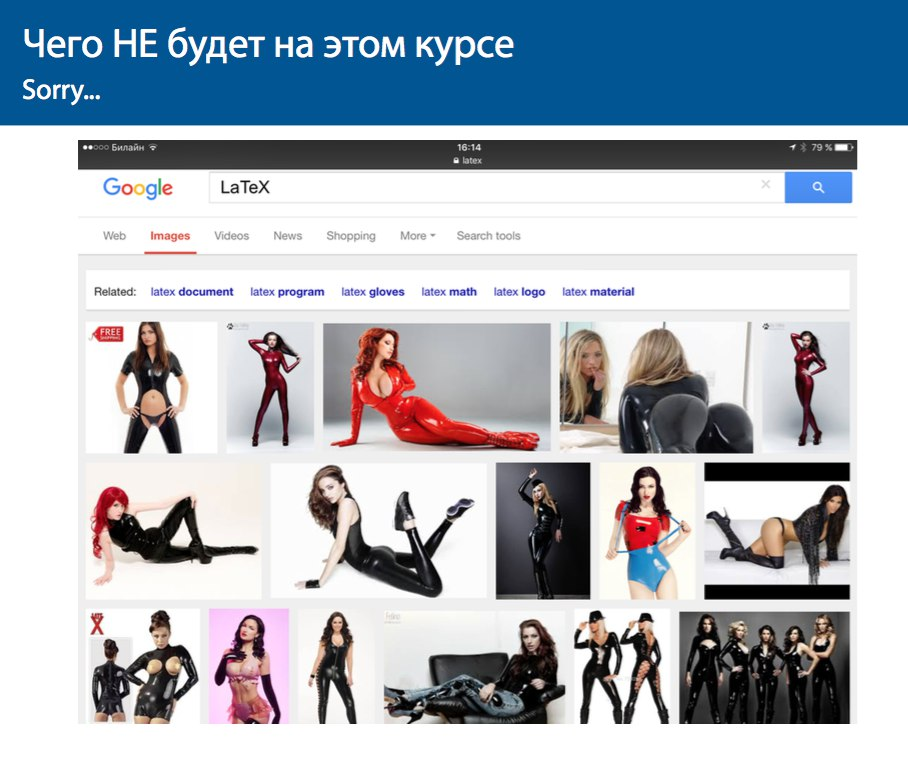
\includegraphics[scale=0.3]{images/latex.jpg}}
\end{frame}

\begin{frame}
	\frametitle{\TeX ~и \LaTeX}
	Тут текст про \TeX
	
	\vfill
	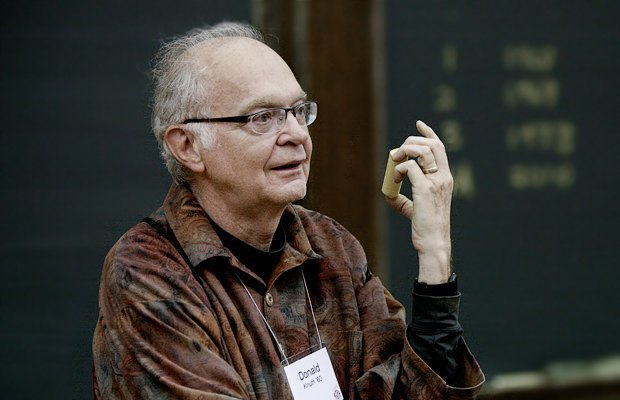
\includegraphics[scale=0.3]{images/knuth.jpg} 
\end{frame}

\begin{frame}
	\frametitle{\TeX ~и \LaTeX}
	Тут текст про \LaTeX
	
	\vfill
	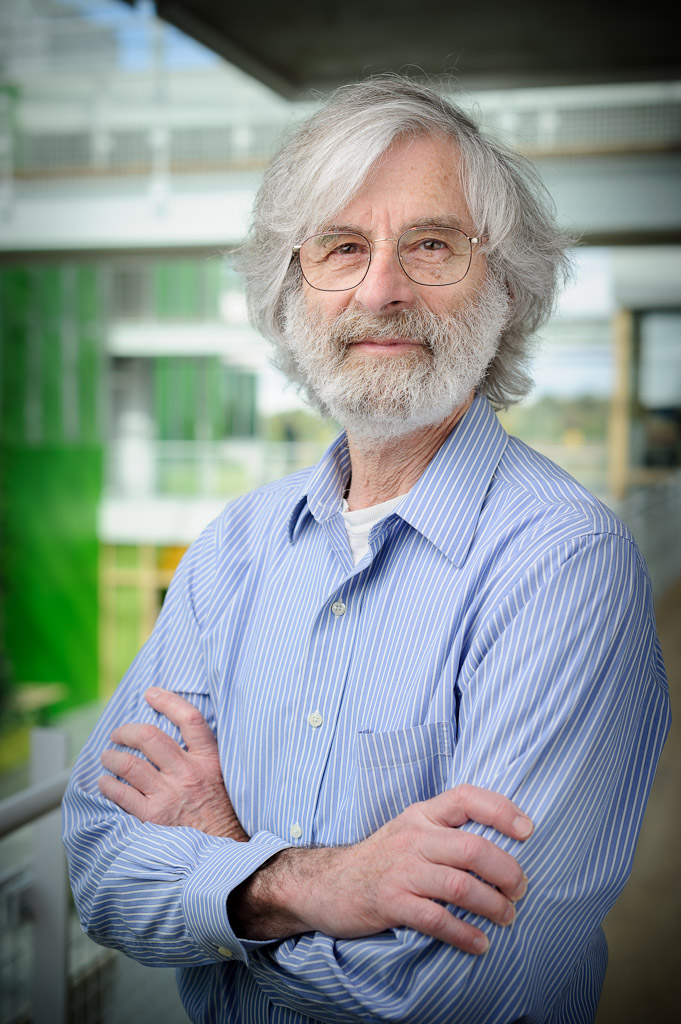
\includegraphics[scale=0.49]{images/lamport.jpg}
\end{frame}

\begin{frame}
	\frametitle{Полезные ссылки и ресурсы}
	Bcnjxybrb 
\end{frame}

\begin{frame}
	\Large {Практика начинается!}
\end{frame}

\begin{frame}
	\begin{center}
		{\Large Спасибо за внимание!}
		
		\vspace{1cm}
		
		Введение в издательскую систему \LaTeX \\
		Семинар-практикум  
				
		\vspace{1cm}
		
		Константин Володин \\
		
		\begin{tabular}{ll}
			\raisebox{-.4\height}{
\includegraphics[scale=0.045]{images/gmail.png}} & {\color{blue}
				\href{mailto:volodin.konstantin@gmail.com}{volodin.konstantin@gmail.com}}\\
		\end{tabular}
		\begin{tabular}{ll}
			\raisebox{-.4\height}{
\includegraphics[scale=0.045]{images/gmail.png}} & {\color{blue}
				\href{mailto:volodin.konstantin@gmail.com}{volodin.konstantin@gmail.com}}\\
		\end{tabular}
		
		\vspace{1cm}
		
		{\small{\today}}
	\end{center}	
\end{frame}



\end{document}